\documentclass[tikz,border=0mm]{standalone}
\usepackage{tikz}
\usetikzlibrary{positioning}
\tikzset{
    mynodee/.style={minimum height=0mm, minimum width=0mm, inner sep=0mm
  },
  mynode/.style={
    draw, circle, minimum height=1.7mm, minimum  width=1.7mm,line width=0.5mm
  },
  rect/.style={
    draw, rectangle, rounded corners, minimum height=7mm, minimum  width=30mm,line
    width=0.5mm, dotted
  }
}

\begin{document}

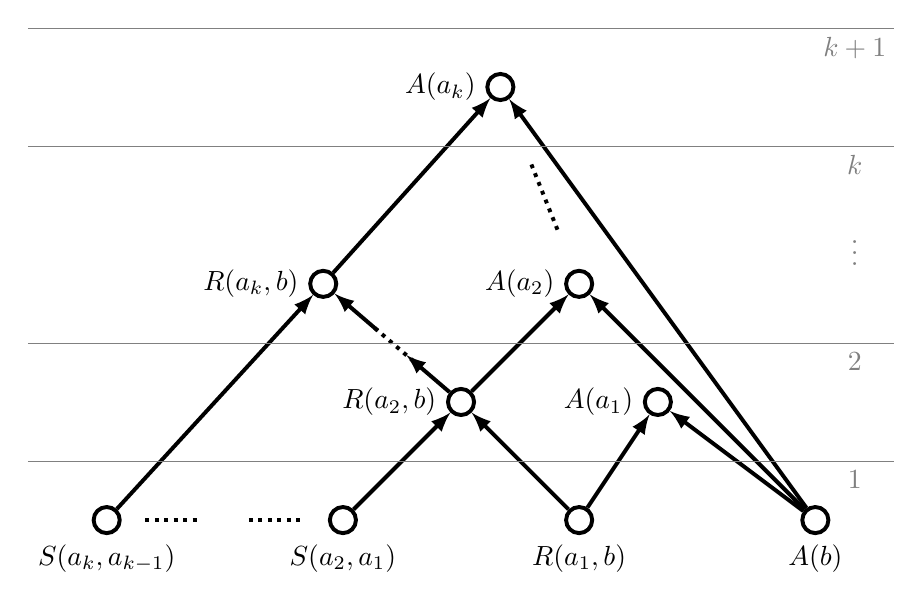
\begin{tikzpicture}
 \node[mynode, label=below:{$S(a_k, a_{k-1})$}] (sakak-1) at (1, 0) {};
 \node[mynodee] (d) at (2.5, 0) {};
 \node[mynode, label=below:{$S(a_2, a_1)$}] (sa2a1) at (4, 0) {};
 \node[mynode, label=below:{$R(a_1, b)$}] (ra1b) at (7, 0) {};
 \node[mynode, label=below:{$A(b)$}] (ab) at (10, 0) {};
 \node[mynode, label=left:{$R(a_2, b)$}] (ra2b) at (5.5, 1.5) {};
 \node[mynode, label=left:{$A(a_1)$}] (aa1) at (8, 1.5) {};
 \node[mynode, label=left:{$R(a_k, b)$}] (rakb) at (3.75, 3) {};
 \node[mynode, label=left:{$A(a_2)$}] (aa2) at (7, 3) {};
 \node[mynode, label=left:{$A(a_k)$}] (aak) at (6, 5.5) {};

 \draw[-latex,line width=0.5mm] (sakak-1) -- (rakb);
 \draw[-latex,line width=0.5mm] (sa2a1) -- (ra2b);
 \draw[-latex,line width=0.5mm] (ra1b) -- (ra2b);
 \draw[-latex,line width=0.5mm] (ab) -- (aa1);
 \draw[-latex,line width=0.5mm] (ab) -- (aa2);
 \draw[-latex,line width=0.5mm] (ab) -- (aak);
 \draw[dotted,line width=0.5mm,shorten >=6mm,shorten <=6mm] (ra2b) -- (rakb);
 \draw[-latex,line width=0.5mm,shorten >=12mm] (ra2b) -- (rakb);
 \draw[-latex,line width=0.5mm,shorten <=12mm] (ra2b) -- (rakb);
 \draw[-latex,line width=0.5mm] (ra1b) -- (aa1);
 \draw[-latex,line width=0.5mm] (ra2b) -- (aa2);
 \draw[dotted,line width=0.5mm,shorten >=8mm,shorten <=5.5mm] (aa2) -- (aak);
 \draw[-latex,line width=0.5mm] (rakb) -- (aak);
 \draw[dotted,line width=0.5mm,shorten >=3mm,shorten <=3mm] (sakak-1) -- (d);
 \draw[dotted,line width=0.5mm,shorten >=3mm,shorten <=3mm] (d) -- (sa2a1);

 \foreach \i/\l in {{0.75/1}, {2.25/2}, {4.75/k}, {6.25/k+1}} {
   \draw[very thin,gray] (0,\i) -- (11,\i) node [below] at (10.5,\i) {$\l$};
  }
  \node[gray] at (10.5,3.5) {$\vdots$};
\end{tikzpicture}

\end{document}
